\documentclass{article}

%Packages
\usepackage{graphicx}
\usepackage{grffile}
\usepackage{float}

%Margins
\usepackage[
margin=2cm,
includefoot
]{geometry}

%Images
\usepackage{graphicx}

\graphicspath{{images/}}

%Headers and Footers
\usepackage{fancyhdr}
\pagestyle{fancy}
\fancyhead{}
\fancyfoot{}
\fancyfoot[R]{\thepage}
\renewcommand{\headrulewidth}{0pt}
\renewcommand{\footrulewidth}{0pt}


%Details
\title{
	Functional Specification
}
\author{Illusion Solutions}

%Document start
\begin{document}
	
	%Title Page
	\newgeometry{top=4.5cm}
	\begin{titlepage}
		\begin{center}
			\line(1,0){300} \\
			[0.1cm]
			\textsc{\Huge
				PowerCloud\\
				Functional Specification
			} \\
			\textsc{\large version 2.0}\\
			[0.1cm]
			\line(1,0){300} \\
			[2.0cm]
			\textsc{\Large
				Illusion Solutions
			} \\
			[3.5cm]
			
		\end{center}
		\begin{flushright}
			\textsc{\Large
				Stuart Andrews\\ 
				12153983\\
				Marc Antel\\
				12026973\\
				Mothusi Masibi\\
				12004589\\
				Brandon Wardley\\
				29005150\\
				[4.0cm]
			}
		\end{flushright}
		\begin{center}
			\today
		\end{center}
	\end{titlepage}
	
	\newpage
	\restoregeometry
	\tableofcontents
	\thispagestyle{empty}
	
	\newpage
	
	\section{Introduction}
	
	The purpose of this document is to describe the functional 
	requirements of the PowerCloud project. This document is an ongoing 
	piece of work, and is updated as the project progresses.
	\section{Vision}
	\textbf{PowerCloud} is a system which allows its users to measure the power consumption of an appliance, store this 
	information on a cloud platform, and view useful reports based on this information via a web interface. The system will 
	allow the storage of important meta-data pertaining to a source's power consumption and which devices the data is taken 
	from. The system is initially intended to be used for internal use and testing by the client, Buhler.\\
	
	The system will consist out of a hardware component, and a software component. The hardware component will be tasked with 
	measuring the current and voltage from an input device, which will be used to perform the power calculations which are 
	required. The hardware device will send this information to a web server. This server will perform any required processing 
	on this information, before posting it to a persistence provider.\\
	
	A user within the system will have access to a number of functions. Users will be able to add and set up new devices, 
	adding to the system, which will send data based on readings from the attached appliance. Additionally, the user can view 
	the data once it has be stored on the persistence provider, and can request reports based off of this data.
	
	\section{Background}
	PowerCloud enables the tracking and monitoring of the power and electricity 
	usage of electrical appliances and machines. PowerCloud could potentially help 
	businesses understand the fluctuations in energy usages and could use this 
	knowledge to optimizes costs in terms of running electrical equipment.
	
	PowerCloud enables a single person to monitor a whole host of appliances at any 
	given time, instead of perhaps having a single engineer observing multiple 
	machines gauges for example. This would speed up the process of determining if 
	a machine is running correctly or if there's a potential problem with it. The 
	foresight that PowerCloud provides could be the difference in spotting a 
	problem in a machine and the destruction of said machine.
	\newpage
	\section{Functional Requirements and Application Design}
	\subsection{Use case prioritization}
	\subsubsection{Application Server}
	\begin{enumerate}
		\item	MQTT Server Startup - Critical
		\item	Firebase Authorisation - Critical
		\item	Validate ID - Important
		\item	Storing Data in Firebase - Critical
	\end{enumerate}
	\subsubsection{Firmware}
	\begin{enumerate}
		\item	Particle Photon Connecting to Server - Critical
	\end{enumerate}
	\subsubsection{Web}
	\begin{enumerate}
		\item	User Add Device - Critical
		\item	Create Firebase Database - Critical
		\item	User Registration - Important
		\item	User Login - Important
		\item	Retrieve Data  - Important
	\end{enumerate}
	\subsection{Use case/Services contracts}
	\subsubsection{Application Server}
	\begin{enumerate}
		\item	MQTT Server Startup
		\begin{enumerate}
			\item  Pre-Conditions
			\begin{enumerate}
				\item  	Server.conf configuration file needs to be present in order for the Server to start listening for incoming MQTT Connection and 
				Publish requests on the correct ports.
				\item	Server throws a MissingConfigFileException if the Server.conf file is not present.
			\end{enumerate}
			\item  Post-Conditions		
			\begin{enumerate}
				\item	Server can receive MQTT requests.
			\end{enumerate}
		\end{enumerate}
	\end{enumerate}
	\subsubsection{Firebase}
	\begin{enumerate}
		\item	Firebase Authorisation
		\begin{enumerate}
			\item  Pre-Conditions
			\begin{enumerate}
				\item	auth.json file needs to be present in order to achieve authorisation for powercloud-bf968.firebaseio.com.
				\item	Device must have authorisation to access Firebase.
				\item	Server throws a MissingAuthorisationFileException.
			\end{enumerate}
			\item  Post-Conditions		
			\begin{enumerate}
				\item	Device can save and retrieve data to and from Firebase.
			\end{enumerate}
		\end{enumerate}
		\item Validate ID
		\clearpage
		\begin{figure}[H]
			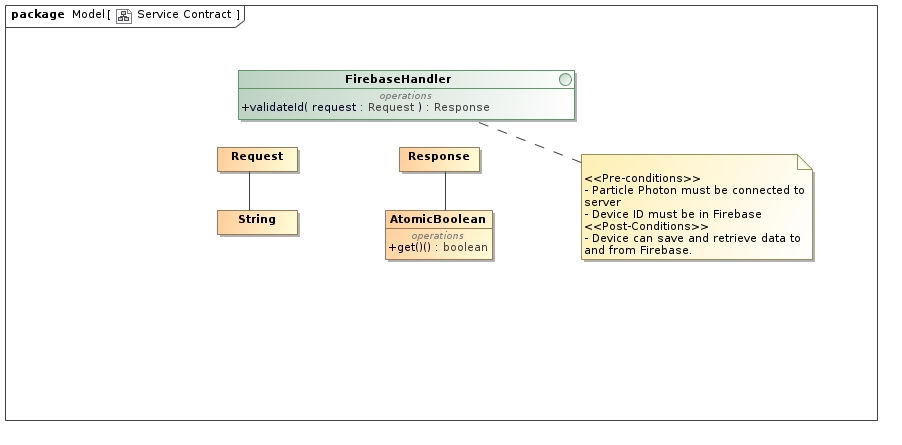
\includegraphics[width=\textwidth]{images/validateIdServiceContract.jpg}
			\caption{Service Contract for validateId \label{overflow}}
		\end{figure}
		\begin{enumerate}
			\item  Pre-Conditions
			\begin{enumerate}
				\item	The Particle Photon must have connected to the server.
				\item	Device ID must be in Firebase, else it will throw a DeviceNotFoundException.
			\end{enumerate}
			\item  Post-Conditions		
			\begin{enumerate}
				\item	The ValidateID function calls the store function, and attempts to store the data.
			\end{enumerate}
		\end{enumerate}
		\item	Storing Data in Firebase
		\begin{figure}[H]
			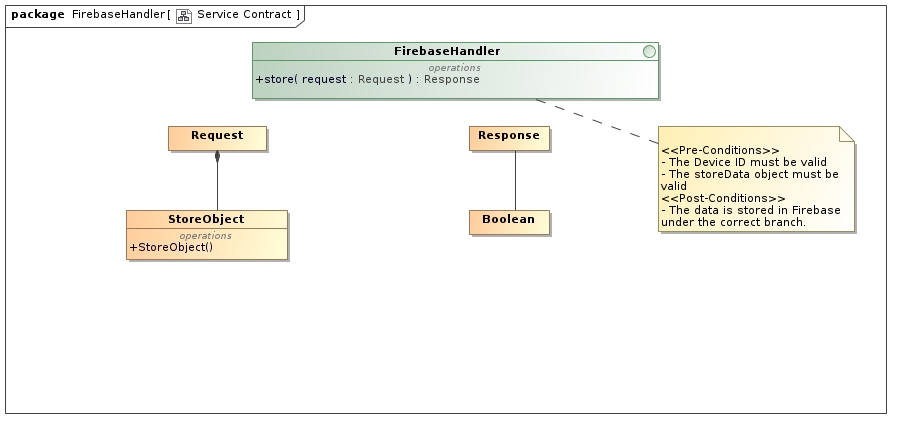
\includegraphics[width=\textwidth]{images/storeServiceContract.jpg}
			\caption{Service Contract for store \label{overflow}}
		\end{figure}
		\clearpage
		\begin{enumerate}
			\item  Pre-Conditions
			\begin{enumerate}
				\item	The Device ID must be valid, before an attempt to store can be made.
				\item	The storeData object must be valid.
				\item	Upon failure a StoreException must be thrown.
			\end{enumerate}
			\item  Post-Conditions		
			\begin{enumerate}
				\item	The data is stored in Firebase under the correct branch.
			\end{enumerate}
		\end{enumerate}
	\end{enumerate}
	\subsubsection{Firmware}
	\begin{enumerate}
		\item	Particle Photon Connecting to Server	
		\begin{enumerate}
			\item  Pre-Conditions
			\begin{enumerate}
				\item	The Photon must have the correct addresses, i.e. port number and ip/domain name.
			\end{enumerate}
			\item  Post-Conditions		
			\begin{enumerate}
				\item	The Photon can then begin transmitting data.
			\end{enumerate}
		\end{enumerate}
	\end{enumerate}
	\subsubsection{Web}
	\begin{enumerate}
		\item	Create Firebase Database
		\begin{enumerate}
			\item  Pre-Conditions
			\begin{enumerate}
				\item	User must have a gmail account.
				\item	User must create their own Firebase account. i.e. powercloud-bf968.
				\item	User must set a password of length 6 and above.
			\end{enumerate}
			\item  Post-Conditions		
			\begin{enumerate}
				\item	User can visit firebase.google.com and view their Firebase Database.
			\end{enumerate}
		\end{enumerate}
		\item	User Registration
		\begin{enumerate}
			\item  Pre-Conditions
			\begin{enumerate}
				\item	User must register with:
				\begin{enumerate}
					\item	namecompany name.
					\item	email address.
					\item	password.
					\item	name of Firebase account i.e. powercloud-bf968.
				\end{enumerate}
			\end{enumerate}
			\item  Post-Conditions		
			\begin{enumerate}
				\item	Firebase creates a user entry.
			\end{enumerate}
		\end{enumerate}
		\item	User Login
		\begin{enumerate}
			\item  Pre-Conditions
			\begin{enumerate}
				\item	User must be registered.
				\item	User must login in with an email address or username, and password.
			\end{enumerate}
			\item  Post-Conditions		
			\begin{enumerate}
				\item	User will have access to all devices, will be able to add and remove devices, and retrieve and observe 
				data.
			\end{enumerate}
		\end{enumerate}
		\item	User Add Device
		\begin{enumerate}
			\item  Pre-Conditions
			\begin{enumerate}
				\item	User must be logged in.
				\item	User must have necessary authorisation.
				\item	User must provide the following details:
				\begin{enumerate}
					\item	Device id.
					\item	Device appliance, i.e. the appliance who's value it will be reading.
					\item	Device name.
				\end{enumerate}
			\end{enumerate}
			\item  Post-Conditions		
			\begin{enumerate}
				\item	A sequential entry, i.e. 0,1,2,3...n, will be made in the Firebase Database.
			\end{enumerate}
		\end{enumerate}
		\item	Retrieve Data
		\begin{enumerate}
			\item  Pre-Conditions
			\begin{enumerate}
				\item	User must be logged in.
				\item	User must have necessary authorisation.
				\item	User must have devices listed, i.e. devices that have already been added.
			\end{enumerate}
			\item  Post-Conditions		
			\begin{enumerate}
				\item	Returns a JSON object from Firebase containing all the data concerning that specific device.
			\end{enumerate}
		\end{enumerate}
		\item	View Device
		\begin{enumerate}
			\item  Pre-Conditions
			\begin{enumerate}
				\item	User must be logged in.
				\item	User must have a list of devices available.
				\item	User must be able to select "View Device" on a device.
			\end{enumerate}
			\item  Post-Conditions		
			\begin{enumerate}
				\item	Returns a page where the user may view data from that device, i.e. Power, Current, Cost and Carbon 
				Emissions.
			\end{enumerate}
		\end{enumerate}
		\item	Device Overview
		\begin{enumerate}
			\item  Pre-Conditions
			\begin{enumerate}
				\item	User must be logged in.
				\item	User must be on the "Overview" page.
				\item	User must enter a date to begin searching from and a date to search to, and hit the search button.
			\end{enumerate}
			\item  Post-Conditions		
			\begin{enumerate}
				\item	Returns a page where the user may view data from all their devices, i.e. Power, Current, Cost and 
				Carbon Emissions totalled per Devices and displayed in pi charts.
			\end{enumerate}
		\end{enumerate}
		\item	Switch Device On/Off
		\begin{enumerate}
			\item  Pre-Conditions
			\begin{enumerate}
				\item	User must be logged in.
				\item	User must view a device
				\item	User must select the settings tab from the overhead bar.
				\item	User must log into their Particle.io account.
				\item	User can click the power button and turn their device on and off.
			\end{enumerate}
			\item  Post-Conditions		
			\begin{enumerate}
				\item	The device in question turns on and off as per the User's request.
			\end{enumerate}
		\end{enumerate}
		\item	Add new Device
		\begin{enumerate}
			\item  Pre-Conditions
			\begin{enumerate}
				\item	User must be logged in.
				\item	User must specify the ID of the new device
				\item	User must specify the name of the new device
				\item	User must specify the task of the new device i.e. What the device is measuring.
			\end{enumerate}
			\item  Post-Conditions		
			\begin{enumerate}
				\item	The user is able to view the device and any of it's readings.
			\end{enumerate}
		\end{enumerate}
	\end{enumerate}
	\newpage
	\subsection{Process specifications}
	\subsubsection{Store Process}
	\begin{figure}[H]
		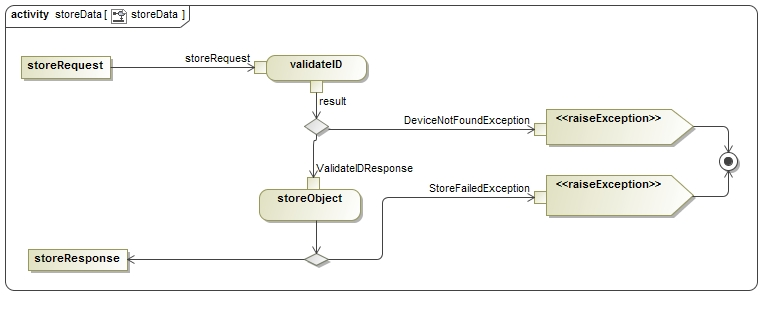
\includegraphics[width=\textwidth]{images/storeData.jpg}
		\caption{Process specification for store \label{overflow}}
	\end{figure}
	\subsubsection{Retrieve All Data Process}
	\begin{figure}[H]
		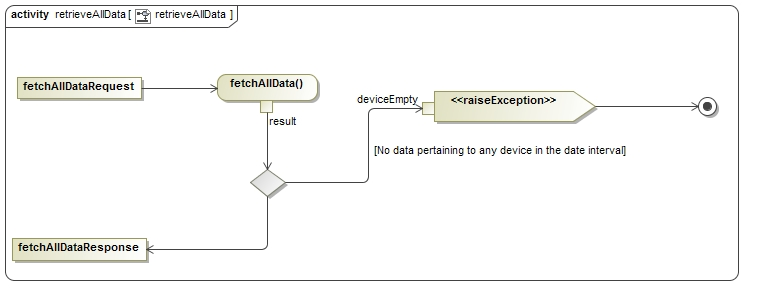
\includegraphics[width=\textwidth]{images/retrieveAllData.jpg}
		\caption{Process specification for retrieve all device data in a interval \label{overflow}}
	\end{figure}
		\subsubsection{Retrieve Data Process}
		\begin{figure}[H]
			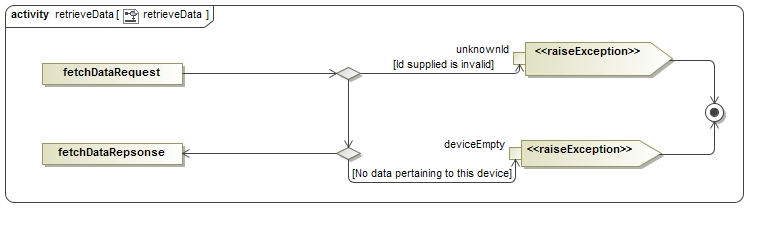
\includegraphics[width=\textwidth]{images/retrieveData.jpg}
			\caption{Process specification for retrieve a specific devices data \label{overflow}}
		\end{figure}
	\subsection{Domain Model}
	\begin{figure}[H]
		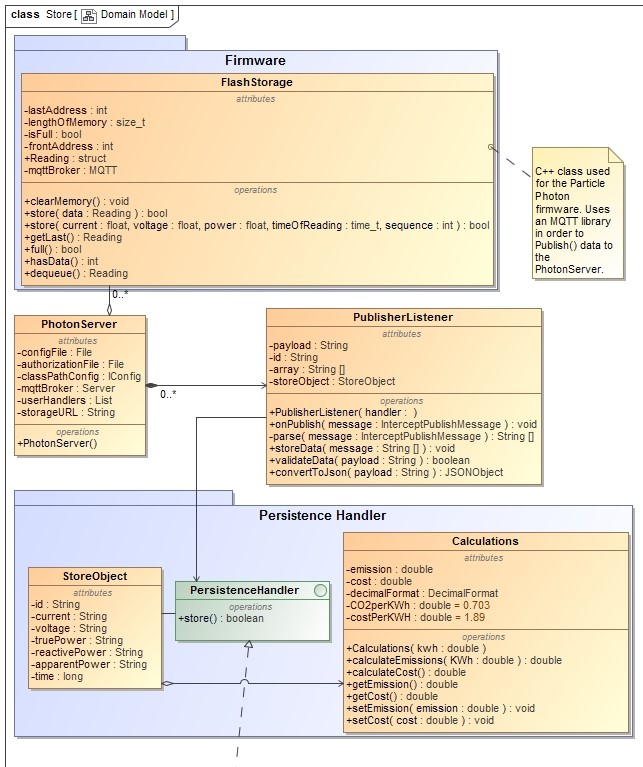
\includegraphics[scale=0.7]{images/Domain Model.jpg}
	\end{figure}
	\begin{figure}[H]	
		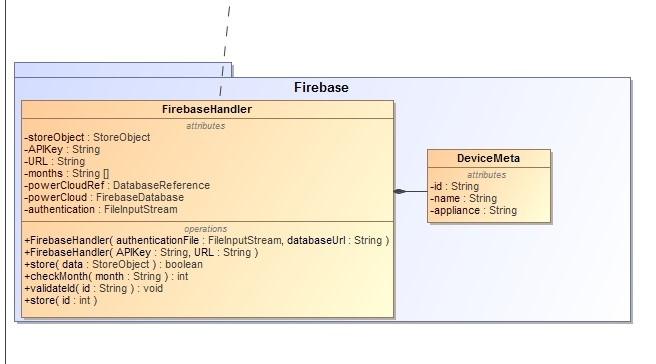
\includegraphics[scale=0.7]{images/Domain Model (2).jpg}
		\caption{Domain Model for PowerCloud \label{overflow}}
	\end{figure}
\end{document} 